\chapter{Proposed solution}\label{sec:solutionProposal}

We have seen that \acrshort{ad} testing is \textit{complex} and that it is difficult to get a good
test coverage (\Cref{sec:adsTestingComplexity}). Furthermore, we have seen that \acrshort{llms} have
\textit{emergent abilities} (\Cref{sec:emergentAbilities}). We therefore propose a tool for
\begin{inparaenum}
    \item running a base \acrshort{ad} test case,
    \item enhancing the test case using \acrshort{llms},
    \item running the enhanced test case,
    and
    \item comparing the results of the two runs.
\end{inparaenum}

This will allow us to learn the extent to which \acrshort{llms} can be applied for enhancing
\acrlong{ad} test cases. We will survey several \acrshort{llms} and evaluate their applicability for
the problem at hand, in light of what we know about \acrshort{llms} (\Nref{sec:llmJungle}).
We want to have a pipeline that is able to process several test cases in succession, in order to get
a substantial dataset.

Let the pipeline tool be known as \hefe.~%\info{This name is naturally just a placeholder.}.
The tool follows a natural pipeline structure. We have some base test cases that
need to be ran in order to get a baseline for the results, we then have to
improve these, and run the improved versions and compare them to their original
versions. The architecture of the tool is visualised in \Cref{fig:hefeArch}.

\begin{figure}[h]
    \centering
    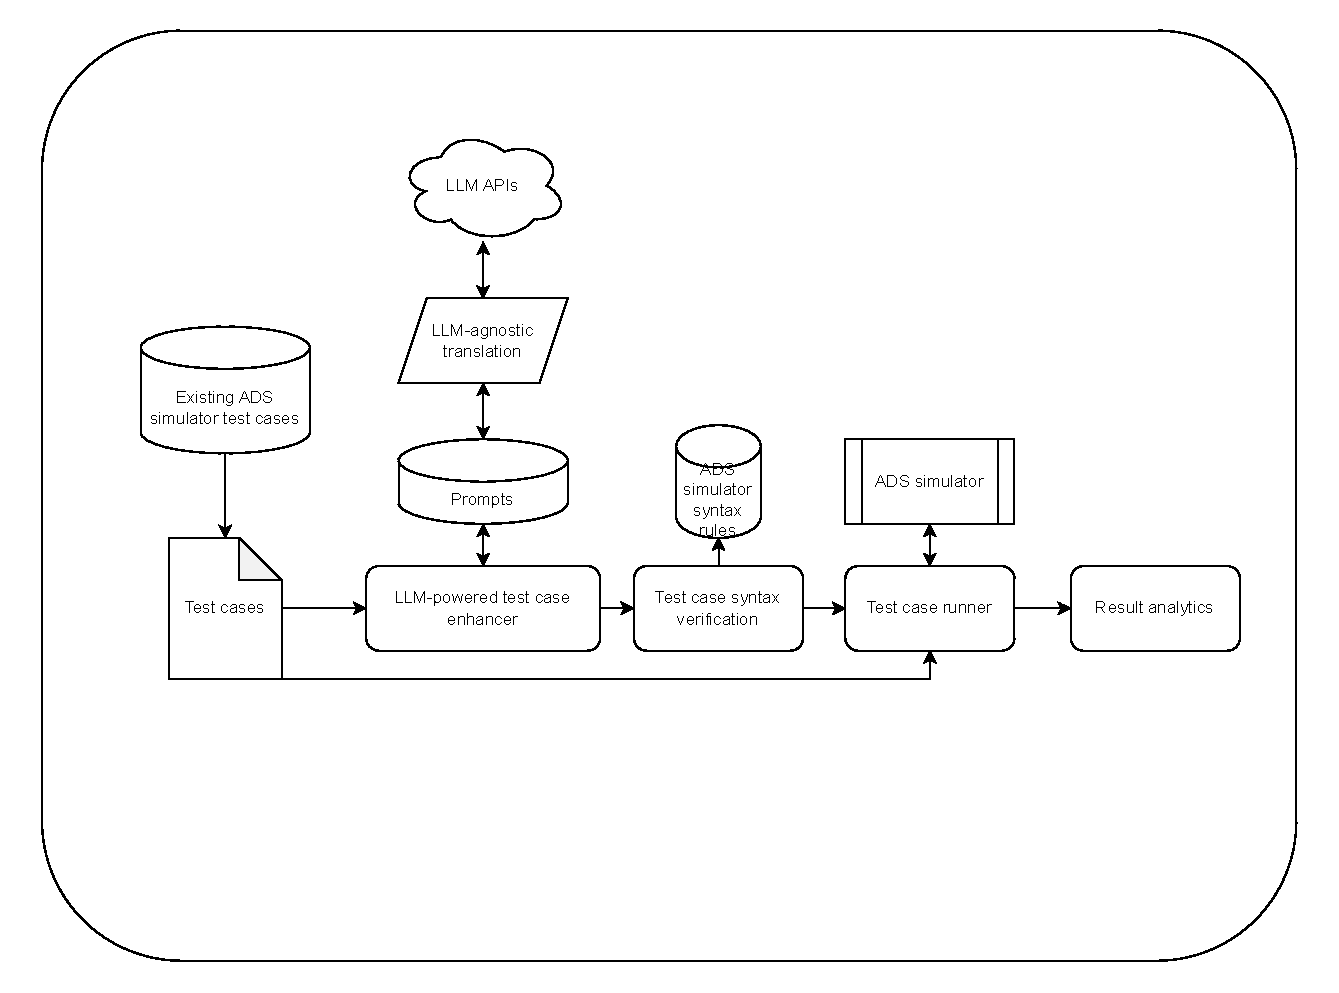
\includegraphics[width=\textwidth]{master-essay-solution-proposal.drawio.pdf}
    \caption{\hefe~pipeline architecture}\label{fig:hefeArch}
\end{figure}

We need to define what requirement we will use for determining the \textit{result} of a test case
run. Without this, we cannot compare it to other test cases.

Furthermore, as outlined in \citeauthor{LLM4AD}, \acrlong{llms} can be applied to several aspects
of \acrlong{ads}. It is not feasible that we focus on \textit{all} these aspects, and as such we
should narrow down our scope. Let us review some of the relevant aspects.

\section*{The applicability of \acrshort{llms} in \acrshort{ad} testing}

\acrlong{ads} are typically modular, as we have seen in \Cref{sec:adsTestingComplexity}.
\acrshort{llms} are applicable to the different modules in different ways as we saw in
\Nref{sec:relatedWork}.
% TODO: Make more specific reference to what part of Related Work

\begin{tcolorbox}[colback=gray!5!white,colframe=gray!75!black,title=User history
        of using \hefe]\label{user-history}
    I have a set of \acrfull{ad} test cases. I provide this set to \hefe. It will run the entire
    set, and generate a baseline of my \acrshort{ad} performance.

    \hefe~will then improve my test cases using \acrlong{llms} and run them again.

    Lastly \hefe~will report how the results differ from running the base and enhanced version of a
    test case.

    This will give me insight into what caused my \acrshort{ad} to fail so that I can look into the
    cause of the error state and uncover underlying faults in the \acrlong{ad}.

\end{tcolorbox}


\section{Implementation language}

The programming language \textsc{Python} is widely used for \acrfull{ad} simulation. It is a high
level language, allowing the user great flexibility and developer experience. For this reason, I will
implement \hefe~using Python.

Python can be optimized using \acrfull{jit} compilers such as Numba~\cite{numba}, which can speed up
our execution times. Libraries such as Joblib provide Python with plug-and-play
meomization, which will allow us to re-use values that have already been
computed, saving time and energy.

\subsection{The room for concurrency}

When evaluating \acrshort{ad} test cases, the test cases are independent of each
other. This means that our problem is \textit{embarrassingly parallelizable}
\footnote{\url{https://en.wikipedia.org/wiki/Embarrassingly_parallel}} and we can
trivially process several test cases in parallel. Due to practical limitations
in Carla, \textit{running} the test cases should however probably be done
sequentially. But \begin{inparaenum}
    \item prompting,
    \item enhancing, and
    \item validating,
\end{inparaenum}
can all be done concurrently. While Python lacks support of traditional threads,
it has some support for multiprocessing
\footnote{\url{https://docs.python.org/3/library/multiprocessing.html}}.

\section{Overview of the components of the \hefe~pipeline}

The pipeline architecture is visualised in \Nref{fig:hefeArch}. Here we
present the major components and their responsibilities


\subsection{Test case enhancement}

\subsubsection{Test case repositories}

We have seen in \Nref{sec:relatedWork} that there are existing repositories of
% TODO: Make more specific reference to what part of Related Work
\acrshort{ad} test cases. These will provide us with \begin{inparaenum}
    \item a baseline,
    and
    \item data onto which we can apply our \acrshort{llm} enhancements.
\end{inparaenum}

\subsubsection{\acrshort{llm} enhancement}\label{sec:llmEnhancement}

The base test cases will individually be enhanced by prompting the
\acrshort{llm}. We will experiment with several \acrshort{llms}.

For performing the actual improvement, it is essential that we \begin{inparaenum}
    \item test several \acrshort{llm},
    \item give clear prompts
    % \info{I'm inclined to find some fitting prompts through trial and error, as such a I do not wish to describe them in detail at this time.}
    and
    \item verify that the returned test case adheres to the strictly necessary
    syntax rules. This last point is important due to our knowledge of
    \acrshort{llms} hallucinating (see \Nref{sec:llmProblems}).
    % TODO: More specific reference to Halucination intead of all LLm problems?
\end{inparaenum}

In order to facilitate testing various \acrlong{llms}, we should employ
\acrshort{llm} agnostic software as a translation layer. This will allow us to
write code for a common interface and test several \acrshort{llms} that may all
have different internal \acrfull{apis} without having to modify our test code
for specific \acrshort{apis}. This \begin{inparaenum}
    \item saves time
    and
    \item makes for more even test conditions \end{inparaenum}. Some pieces of software providing
this type of functionality include
\textsc{aisuite}\footnote{\url{https://github.com/andrewyng/aisuite}}, RamaLama from
RedHat\footnote{\url{https://github.com/containers/ramalama}}, and the MIT licensed
Ollama\footnote{\url{https://github.com/ollama/ollama}}, both supporting a plethora of
\acrlong{llms}.

\textsc{guidance}\footnote{\url{https://github.com/guidance-ai/guidance}} is a
framework for limiting the room in which \acrshort{llms} may operate, which
might be useful if we run into issues with excessive hallucination.


\subsubsection{Enhanced test case validation}

We must expect the \acrshort{llm} to hallucinate to some extent (\Cref{sec:llmHallucination}). We
therefore propose to verify the format of the enhanced file before running it.

As we saw in the section for \Nref{sec:adsScenarioFormats}, there exists several formats for
\acrshort{ad} scenarios. In order to verify that the syntax of our enhanced test
case is valid, we simply need to apply the syntax rules of our format. 

The CommonRoad format is XML-based~\cite[720]{commonRoadOG} and as such we can
to some extent assess the degree of hallucination by parsing the XML structure.
Futhermore, it has an exhaustive Python library with several utilities\footnote{\url{https://pypi.org/user/commonroad/}}.

OpenSCENARIO exists both as XML and a domain-specific language (DSL). If we
utilise the XML version, we can apply the same methodology as for the CommonRoad
format. If using the DSL version, one way
the OpenSCENARIO format can be verified is by using free
online cloud services such as this offering from AVL
\footnote{\url{https://smc.app.avl.com/validation}}. We should however strive for
running a local verification service to \begin{inparaenum}
    \item save time and compute,
    and
    \item preserve data privacy.
\end{inparaenum}
Besides, it is generally a good idea to limit the number of external dependencies\footnote{Note for
    example how LGSVL\cite{lgsvl} was shut down, preventing projects such as DeepScenario of
    \citeauthor{DeepScenario} to be further developed on the original platform.}.

\subsection{Test case running and evaluation}

\subsubsection{Test case runner}

The system will automatically run all
our base test cases using an \acrshort{ad} simulator, and collect data points to get a baseline. It
will later also run the mutated \acrshort{llm}-enhanced versions of the base cases.

We have already ran the test cases in their base form. We will now run their
improved versions in order to compare them to see what effect the \acrshort{llm}
enhancement (see \Cref{sec:llmEnhancement}) has had.

For the reasons we have seen in~\Cref{sec:simulatorOverview}, we want to run our
test cases on Carla. It is the best offering as it is open source, under active
development and has a feature rich Python \acrshort{api}.

\subsubsection{Test case improvement evaluation}\label{sec:testCaseEval}

We saw in \Cref{sec:adsMetrics} that there are several metrics for assessing
\acrshort{ads}. We will use these metrics when evaluating our improvements.

\subsubsection{Test case result reporting}

We will compare the results from running
the baseline unmodified test case and comparing it with the results from
running the \acrshort{llm}-enhanced version and returning to the user. Ideally with
some automatic analysis of the results.

Having ran both the base test case and its enhanced counterpart, we have
results. The results will be stored in \acrfull{csv} files, allowing \begin{inparaenum}
    \item further analysis in Python/Jupyter,
    and
    \item easy translation to \LaTeX tables for the final report.
\end{inparaenum}

This is the final step of the envisioned pipeline. Where we have our result, and
need to analyse them.

This last step has great opportunities for being scoped up to a fully integrated
test suite which allows for both running test cases and analysing the results in
a \acrfull{gui}. But we should focus on the prior steps for now, only creating a
\acrshort{gui} if there is sufficient time towards the end of the project to
focus on such non-\acrshort{llm} related topics.

Initially, the results will consist of numerical comparison of the
\acrshort{csv}s with regard to the relevant metrics outlined in
\Nref{sec:testCaseEval}.
